\chapter{Fundamentação Teórica}
\label{c.fundamentacao}

\section{Botnets}

\textit{Botnets} são redes de computadores comprometidos, que são usados para cometer vários tipos de crimes virtuais, entre eles ataques de negação de serviço (\textit{DDoS}), disseminação de vírus, fraudes de cliques para geração de dinheiros em propagandas \textit{online}, e obtenção de dados pessoais \cite{ianelli2005botnets}.

Uma \textit{Botnet} pode ser vista como o conjunto de três agentes: \textit{bots}, máquinas que foram infectadas por um \textit{malware}; um \textit{botmaster}, pessoa capaz de controlar os \textit{bots} de modo que eles executem ações determinadas por ele sem o consentimento de seus respectivos donos; e o Sistema de Comando e Controle, estrutura responsável por distribuir os comandos do mestre para todas as máquinas comprometidas. \cite{miller2016role}

Existem três topologias principais para as botnets, de acordo com o tipo de Comando e Controle utilizado \cite{jang2009analysis}. Uma \textit{botnet} centralizada possui um servidor central ao qual o mestre envia os comandos, que depois repassa-os para todos os bots conectados. Elas se diferenciam pelo tipo de protocolo utilizado, sendo HTTP e IRC os mais utilizados.

Já as descentralizadas não possuem uma estrutura central, utilizando ao invés disso comunicações \textit{peer to peer} (P2P) entre suas máquinas para as transmissões de mensagens. 

Há ainda uma abordagem híbrida, que diferencia as máquinas infectadas entre servos e clientes, sendo as primeiras responsáveis por receber e enviar as mensagens e as últimas por executar os comandos recebidos. 

A figura \ref{f.topologias} ilustra as diferentes topologias, aonde I representa uma \textit{botnet} centralizada, II descentralizada, e III uma aplicação híbrida.

\begin{figure}[h]
\caption{\small Arquiteturas de Botnet.}
\centering
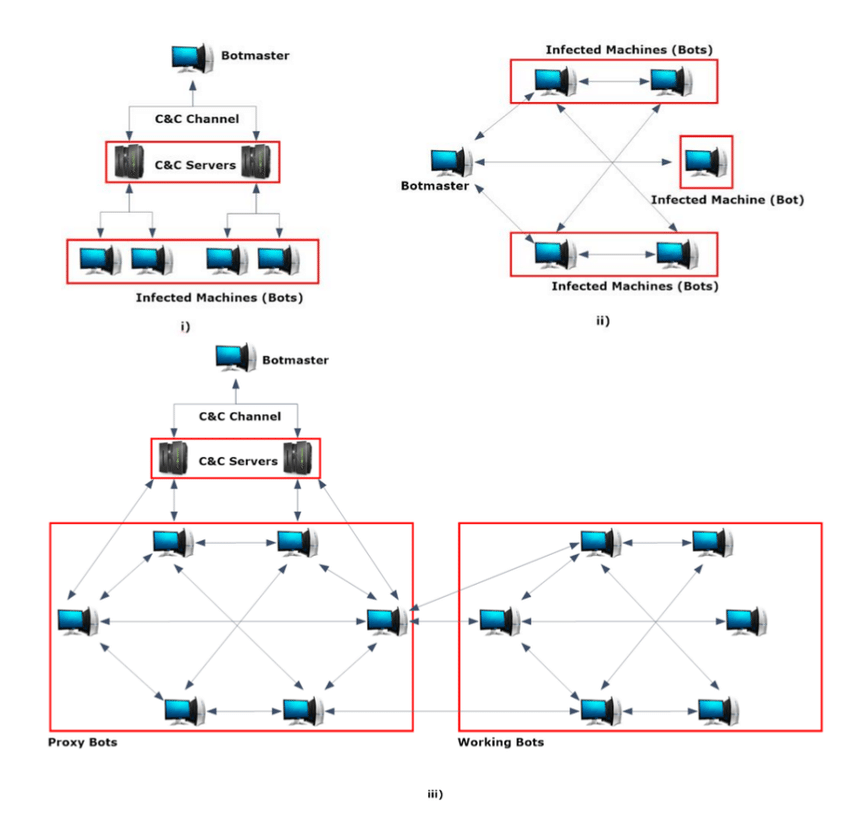
\includegraphics[scale=0.25]{figs/topologias.png}
\label{f.topologias}
\legend{\small Fonte: \cite{imagembotnets}.}
\end{figure}

As \textit{botnets} descentralizadas, por não possuírem uma estrutura central de comando, são mais difíceis de serem rastreadas e derrubadas, enquanto as centralizadas são mais suscetíveis a serem derrubadas, tendo em vista que se o Servidor de C\&C for desativado, a \textit{botnet} deixa de funcionar. \cite{feily2009survey}

Por outro lado, as \textit{botnets} centralizadas são muito mais confiáveis e eficientes na questão da comunicação, enquanto as P2P apresentam problemas de latência que acabam diminuindo o poder de seus ataques. Tendo isso em vista, as topologias centralizadas ainda são utilizadas pela sua facilidade de utilização e gerenciamento, além da baixa latência \cite{12d2f5d1eba245f7bc2acc7487941bd7}. Dentre estas, se destacam as que utilizam o protocolo IRC e HTTP.

O Protocolo \textit{Internet Relay Chat} foi desenvolvido para ser utilizado em aplicações de trocas de mensagens em grupo \cite{oikarinen1993internet}. Ele é baseado num modelo de cliente-servidor, aonde um processo funciona como um ponto central, guardando o estado global de todos os outros clientes conectados a ele. Devido a um grande número de aplicações \textit{open-source} baseadas no protocolo IRC, sua implementação acaba sendo muito mais fácil, sendo esse o motivo pelo qual é o mais prevalente historicamente, e o motivo de ser o foco deste estudo. \cite{abu2006multifaceted}

O ciclo de vida de uma \textit{botnet}, segundo \cite{leonard2009framework}, pode ser descrito em quatro passos:

\begin{itemize}
    \item Infecção: nesta etapa, o \textit{botmaster} age infectando várias máquinas com \textit{malwares}, incorporando-as desta maneira à rede;
    \item Ambiente de Comando e Controle: depois de infectada, uma máquina estabele então uma conexão com o Servidor de C\&C, ficando à disposição do mestre para que quando ele desejar, possa enviar uma mensagem para o Servidor, e através deste a ordem é então repassada para todos os \textit{bots} conectados à sua rede;
    \item Ataque: depois que os \textit{bots} recebem as ordens, eles passam então a executar aquilo que foi determinado pela instrução enviada, como enviar \textit{e-mails} de \textit{spam}, por exemplo;
    \item Pós-Ataque: depois que o ataque foi concluído, alguns \textit{bots} podem ser descobertos, levando a uma remoção do vírus e consequentemente, a remoção da máquina da \textit{botnet}. Sendo assim, o foco do mestre é executar a manutenção da rede, e por fim focar no recrutamento de novas máquinas, ponto aonde o ciclo recomeça.
\end{itemize}

Na área de detecção de botnets, têm se destacado muito por sua eficiência técnicas baseadas na mineração de dados, utilizando algoritmos de ML, como observado em \cite{feily2009survey}. A maioria destas técnicas de detecção costumam trabalhar com fluxos de redes, ao invés de pacotes isolados, devido ao fato dos primeiros apresentarem uma possibilidade muito maior de características a serem utilizadas \cite{beigi2014towards}. 

Muitos estudos têm sido feitos nos últimos anos com base nessas técnicas, explorando várias abordagens presentes na literatura de ML, variando desde a utilização de técnicas clássicas como por exemplo o algoritmo de Regressão Logística \cite{logregbot}, até o uso de técnicas mais recentes da área de \textit{Deep Learning}, através da implementação de Redes Neuras Artificiais Convolucionais, como estudado em \cite{rna1} e \cite{rna2}.

\section{Machine Learning}

\textit{Machine Learning} é uma subárea da IA que busca desenvolver algoritmos capazes de extrair conhecimento com base em dados, através da junção de conceitos de Estatística e Ciência da Computação \cite{James:2014:ISL:2517747}. 

Existem dois tipos principais de algoritmos de ML, os algoritmos supervisionados e não-supervisionados.

\subsection{Supervisionado e Não-supervisionado}

Na área de ML supervisionado, são fornecidos os dados de entrada e os dados de saída respectivos, e com base nestes, o algoritmo busca interpretar e buscar padrões nestes dados que possa diferenciá-los. 

Dentro do contexto de algoritmos de ML supervisionados, que é o foco deste trabalho, existem dois tipos de problema principais: Regressão e Classificação.

Problemas de Regressão são capazes de predizer variáveis quantitativas, ou seja, valores numéricos. Um exemplo seria encontrar o ganho anual de uma pessoa de acordo com a escolaridade, idade e local de residência. \cite{muller2017introduction} 

Já para o caso onde tenta-se predizer uma variável qualitativa, ou seja, encontrar a qual classe $C_{n}$ pertence algo dado um conjunto de $n$ classes, têm-se um problema de Classificação. Para casos onde $n=2$, têm-se uma classificação binária, e quando $n>2$, uma classificação multi-classe.

Já em métodos não-supervisionados, as classes dos dados não são passadas ao algoritmo, de maneira que ele busca identificar padrões e relações entre eles, procurando alguma informação possa ser obtida delas. 

Para isso, utilizam-se principalmente as chamadas técnicas de clusterização, que buscam separar os dados em vários grupos de acordo com suas características observadas no conjunto de dados. \cite{muller2017introduction} 

\subsection{Fases de treinamento e teste}

Na área de ML costuma-se utilizar dois conjuntos de dados diferentes na fase de criação de modelos: conjunto de teste e conjunto de treino. O primeiro é utilizado pelo algoritmo para aprender as relações entre os dados, e o de teste para validar a sua eficiência.

Para que se obtenham esses conjuntos, uma prática comum é utilizar a técnica de \textit{Holdout}, que separa uma parte do conjunto de dados para que seja utilizada para teste, enquanto o resto é usado para treinar o modelo. Geralmente isso é definido através de uma proporção, como 70\% do conjunto para teste e 30\% para treino, por exemplo. \cite{van2010process}

Utilizando essa abordagem, espera-se observar que o modelo treinado seja generalizado, capaz de prever dados os quais nunca tenha trabalhado antes da maneira correta. No entanto, isto pode não ocorrer devido a:

\begin{itemize}
    \item Overfitting: ocorre quando o modelo fica muito sensível a certas particularidades do conjunto de treinamento. Isto costuma ocorrer em modelos mais complexos que utilizam um número muito grande de características.
    \item Underfitting: ocorre quando o modelo, por ser muito simples, não é capaz de aprender as características dos dados, e dessa maneira falha em apresentar os resultados esperados. 
\end{itemize}

O desafio na área de ML então é obter um modelo que esteja bem balanceado, não sendo nem muito simples nem muito complexo, de modo a evitar um dos problemas descritos acima. Para isto, podem-se utilizar várias técnicas, dentre elas se destacando o \textit{Cross Validation}, que buscam medir a generalização dos dados \cite{muller2017introduction}.

A técnica de CV baseada em k-folds consiste em separar o conjunto de treinos em k subconjuntos de tamanhos iguais, aonde cada um será usado para treinar um modelo diferente . Estes modelos então são verificados alternando o conjunto de treino e utilizando os outros $k-1$ como teste, e a performance do algoritmo é obtida através da média das performances individuais. 

Algo importante de se notar também é a distribuição do número de amostras. De maneira geral, classificadores costumam ser muito mais efetivos quando trabalham com dados que se encontram balanceados, tendo sua efetividade diminuída caso contrário. \cite{yap2014application}

Neste contexto, podem ser aplicadas duas técnicas: \textit{Oversampling} e \textit{Undersampling}, que buscam aumentar ou diminuir, respectivamente, o número de amostras de uma classe específica de maneira a deixar o conjunto balanceado. A técnica de \textit{Oversampling} costuma ser mais trabalhosa por envolver a criação e adição de novos dados ao conjunto. 

Por fim, outro conceito importante para a generalização dos algoritmos é o dos hiper-parâmetros. Alguns algoritmos possuem parâmetros especiais que definem o seu desempenho e performance, e enquanto alguns algoritmos trabalham bem com seus valores padrão, para outros é necessário executar testes para encontrar os valores ótimos a serem passados. 

Neste contexto, utiliza-se a técnica de \textit{Grid Search}. Esta técnica consiste em testar todas as combinações possíveis de um certo conjunto de valores e verificar qual delas gera o melhor modelo possível \cite{bergstra2012random}.  É possível utilizá-la em conjunto com a técnica de CV para obter um nível de confiabilidade maior.

\subsection{Métricas}

Para se medir a eficiência de um algoritmo, pode-se classificar cada uma de suas predições dentro de quatro possibilidades: Verdadeiro Positivo (VP), Verdadeiro Negativo (VN), Falso Positivo (FP), Falso Negativo (FN). Estes dados são convenientemente agrupados para melhor visualização na chamada Matriz de Confusão. \cite{flach2003geometry}

\begin{figure}[h]
\caption{\small Exemplo de Matriz de Confusão.}
\centering
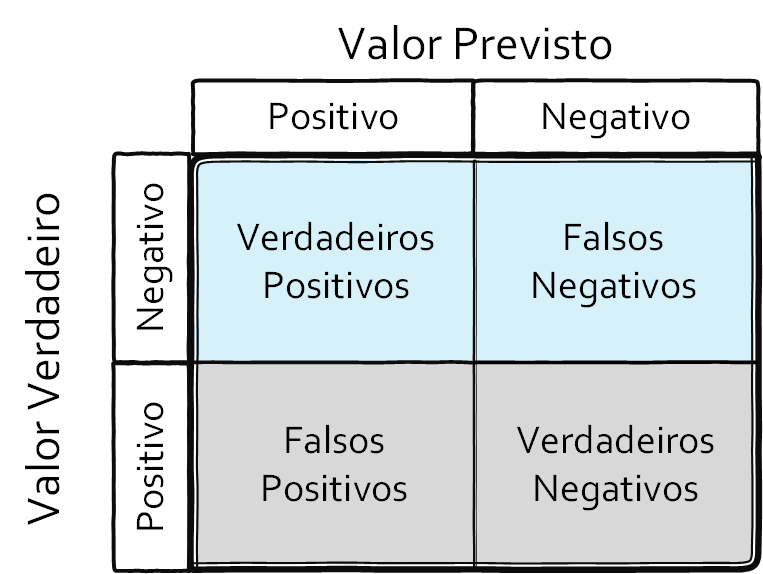
\includegraphics[scale=0.3]{figs/matrizconf.png}
\label{f.matriz-conf}
\legend{\small Fonte: \cite{matriz}.}
\end{figure}

A partir desses dados, é possível obter alguns valores que indicam a eficiência do algoritmo, os quais se destacam:

\begin{itemize}
    \item Precisão: $\frac{VP}{(VP + FP)}$
    \item Recall: $\frac{VP}{VP + FN}$
    \item F-score: $\frac{2 . Precisao . Recall}{(Precisao + Recall)}$
    \item Acurácia: $\frac{VP + VN}{VP + VN + FP + FN}$
    
\end{itemize}

\subsection{Algoritmos}

Nesta seção, serão apresentados os algoritmos da área de ML estudados para a execução deste trabalho.

\subsubsection{Naive Bayes}

Naive Bayes é um classe de algoritmos de ML que possuem sua fundação no Teorema de Bayes. Possui o nome \textit{Naive}, pois é baseado na suposição de que todas as características do problema são independentes umas das outras, algo que muito raramente acontece na grande maioria das aplicações do mundo real.

No entanto, apesar de sua suposição "inocente", classificadores NB são um dois mais eficientes e efetivos algoritmos da área de ML, sendo que se destacam de maneira maior na área de classificação de textos. \cite{zhang2004optimality}

Dada uma classe c, e um conjunto de características $F = x_{1},x_{2},...,xn$, a relação entre elas com base no Teorema de Bayes pode ser descrita da seguinte fórmula:

\begin{equation}
\label{e.bayes}
P(c,F)=\frac{P(F|c)P(c)}{P(F)},
\end{equation}

e a suposição \textit{naive} de que todas as variáveis são independentes umas das outras implica que probabilidade de uma variável dado o valor da classe não depende do valor das outras variáveis do conjunto. Isso pode ser representado da seguinte forma:

\begin{equation}
\label{e.naive}
P(F,c)=P(x_{1},x_{2},...,x_{n}|c)=\Pi_{i=1}^n P(xi|y)
\end{equation}

ou seja, a probabilidade do conjunto F sobre c pode ser representada pelo produto das probabilidades individuais de cada característica $x_{i}$ do conjunto sobre uma classe.

Sendo assim, é possível obter uma equação para Naive Bayes como se segue:

\begin{equation}
\label{eq_final}
r = arg max_{r}P(c)\Pi_{i=1}^n P(x_{i}|y)
\end{equation}

que mostra que o rótulo de uma entrada r será atribuído verificando para qual valor de classe c é obtido uma maior probabilidade com base no conjunto de características do problema.

O que vai diferenciar os tipos de algoritmos de Naive Bayes é o modo como $ P(x_{i}|y)$ é calculado, ou seja, qual o tipo de distribuição que será usada. Estas podem ser Multinomial, Gaussiana ou Bernoulli \cite{Metsis06spamfiltering}. 

\subsubsection{Support Vector Machines}

O algoritmo de \textit{Support Vector Machines} foi criado na década de 90 por \cite{cortes1995support}, e desde então vem recebendo muita atenção da comunidade de ML por seu alto desempenho. Ele foi pensado inicialmente como um classificador binário, no entanto, muitas extensões foram desenvolvidas que permitem o uso da técnica para problemas de classificação de mais de uma classe e para regressão.

A ideia básica do SVM é encontrar um hiperplano ótimo que seja capaz de dividir os dados em duas regiões, de maneira que cada uma delas contenham dados de uma só classe. A equação geral de um hiperplano de dimensão $n$ é demonstrada a seguir:

\begin{equation}
\label{e.hyperplane}
\beta_{0} + \beta_{1}x_{1} + \beta_{2}x_{2} + ... = \beta_{n}x_{n} = 0
\end{equation}

aonde $x_{1},...,x_{n}$ representam as coordenadas de um certo ponto no ${\textrm I\!R}^{n}$ e $\beta_{1},...,\beta_{n}$ são constantes. 

Considerando que para um ponto $x_{n}$ que obedeça a igualdade, este ponto está localizado exatamente acima do hiperplano, o objetivo do algoritmo então é que, dado um problema que possui dados de duas classes $c_{1}$ e $c_{2}$, todos os pontos de uma destas tenha o seguinte comportamento  

\begin{equation}
\label{e.hyperplane-div1}
\beta_{0} + \beta_{1}x_{1} + \beta_{2}x_{2} + ... = \beta_{n}x_{n} > 0
\end{equation}

enquanto para a outra classe seja observável que

\begin{equation}
\label{e.hyperplane-div2}
\beta_{0} + \beta_{1}x_{1} + \beta_{2}x_{2} + ... = \beta_{n}x_{n} < 0
\end{equation}

ou seja, cada classe é encontrada somente em uma região, cada uma de um lado do hiperplano. Para definir a localização deste, busca-se um local onde a distância entre os pontos mais próximos do hiperplano de cada classe, neste contexto denominada margem, seja maximizado. Esta técnica é conhecida como \textit{Marginal Margins Classifier}
\cite{James:2014:ISL:2517747} A figura \ref{f.hiperplano-svm} ilustra a ideia básica destes conceitos.

\begin{figure}[ht]
\caption{\small Hiperplanos no conceito de SVM.}
\centering
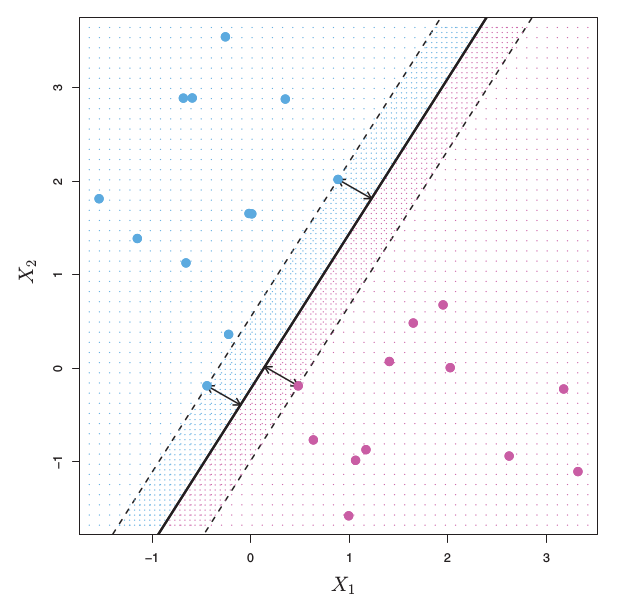
\includegraphics[scale=0.40]{figs/svm-plano.png}
\label{f.hiperplano-svm}
\legend{\small Fonte: \cite{James:2014:ISL:2517747}.}
\end{figure}

No entanto, um caso de dados totalmente capaz de ser separado linearmente é muito raro de ser obtido em uma situação real. Tendo isso em vista, pode ser utilizada uma abordagem diferente, \textit{Soft Margins Classifier} aonde é permitido que pontos estejam localizados não só na região da margem, mas inclusive do lado errado do hiperplano. 

Porém existem ainda os casos aonde os dados não possuem uma distribuição linear, e sendo assim não é possível estabeler um hiperplano entre as classes. Porém, estes dados podem ser separáveis em um espaço de maior dimensão, como demonstrado na próxima imagem \cite{kim2013everything}. 

Depois de obtido o plano no espaço de maior dimensão, este pode ser projetado na dimensão anterior e assim se consegue um hiperplano divisor. Porém, o processo dessas transformações é muito caro computacionalmente, e neste contexto se faz útil a utilização do chamado \textit{Kernel Trick}.

\begin{figure}[ht]
\caption{\small Caso de uso de transformação em SVM.}
\centering
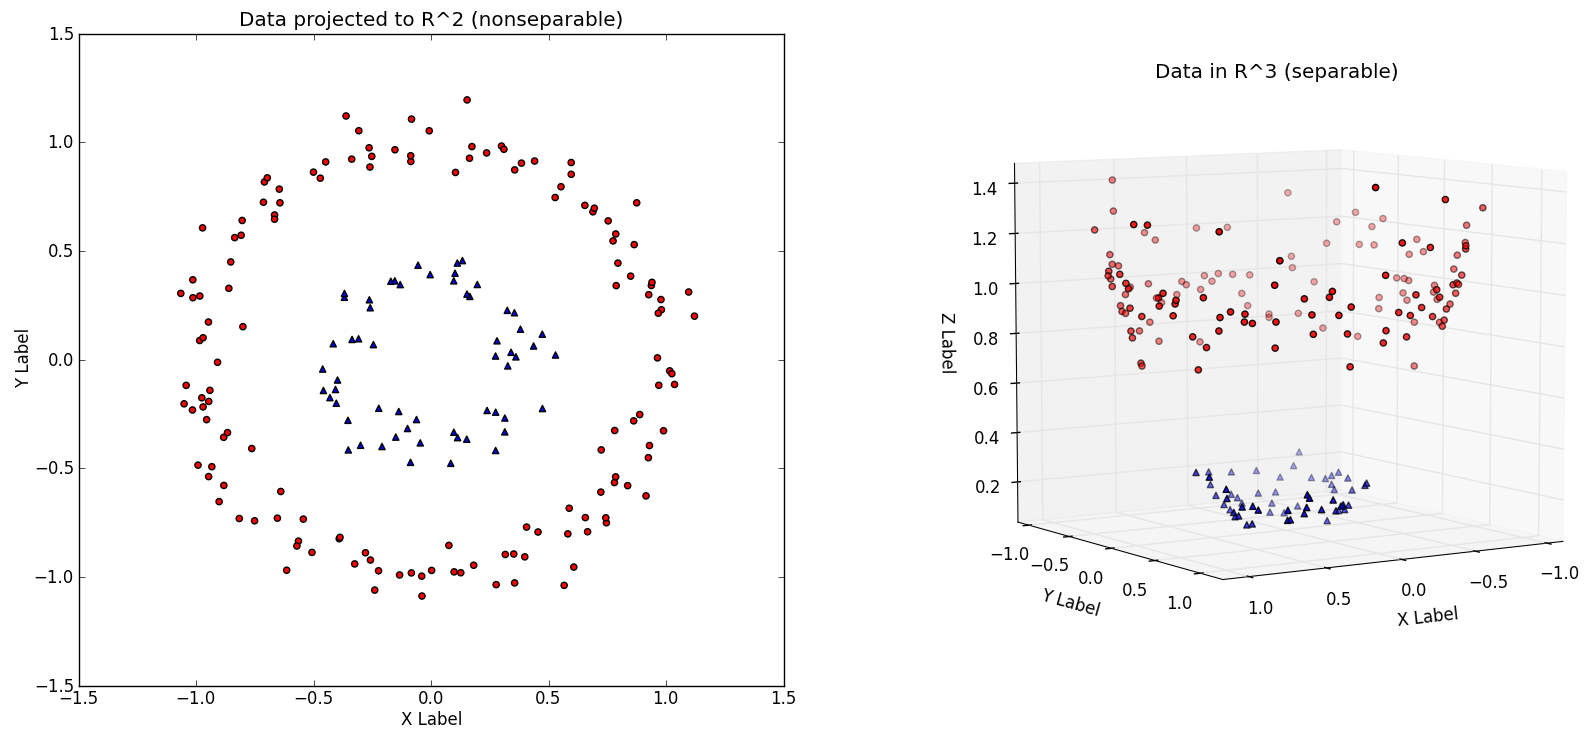
\includegraphics[scale=0.40]{figs/svm-2dto3d.png}
\label{f.svm-transformacao}
\legend{\small Fonte: \cite{kim2013everything}.}
\end{figure}

É possível observar através de comprovações matemáticas, que os resultados do algoritmo de SVM são obtidos através do produto escalar entre seus dados \cite{jordan2004kernel}. Neste contexto, são utilizadas as funções Kernel, que são capazes de calcular o produto escalar de dois vetores, representado por $<x,x'>$, no Rn em um espaço Rm, onde $m > n$, sendo assim capaz de calcular hiperplanos de maneira muito barata computacionalmente.

As funções Kernel mais utilizadas neste contexto são mostradas na tabela \ref{t.kernels}.

\begin{table}[h]
\centering
\begin{tabular}{|c p{5cm}|l p{5cm}}
\hline
\textbf{\small Nome} & \textbf{\small Função Kernel}\\\hline \hline
{\small Linear} & {\small $<x,x'>$}\\\hline
{\small Polinomial} & {\small $(\gamma<x,x'> + r)^{d}$}\\\hline
{\small Radial Basis Function} & {\small $\exp(-\gamma \parallel x - x' \parallel^{2})$}\\\hline
{\small Sigmoidal} & {\small $\tanh(\gamma<x,x'> + r)$}\\\hline
\end{tabular}
\caption{Funções Kernel utilizadas em SVM.}
\label{t.kernels}
\end{table}

Uma grande desvantagem do SVM é que eles exigem que seus hiper-parâmetros sejam muito bem otimizados para que ele tenha um bom desempenho, assim exigindo um estudo maior para ser utilizado. 

O Hiper-parâmetro C, constante de margens suaves, é comum a todos os Kernels e determina o peso da minimização dos erros no conjunto de treinamento. Além disso, como observado na tabela acima, alguns Kernels possuem valores específicos que devem ser determinados como $\gamma$, $r$ e $d$ (\textit{degree}) \cite{lorena2007introduccao}.

\subsubsection{Árvores de Decisão}

Árvores de decisão, no contexto de ML, são métodos que se assemelham muito a fluxogramas, pois busca através de perguntas do tipo \textit{if-else} encontrar um certo resultado \cite{harrington2012machine}.

Para definir os testes e divisões feitos, as árvores de decisão trabalham com uma abordagem denominada \textit{splitting}, onde de maneira recursiva as os dados são divididos em regiões menores, de modo que eles fiquem de maneira mais dividida possível.

Uma árvore de decisão possui três tipos de nós:

\begin{itemize}
    \item Nó raiz: o nó inicial da árvore, por onde começa o processo de divisão;
    \item Nós de decisão: nós que contêm cada uma das decisões feitas pelo algoritmo, definem através de comparações qual o caminho a ser percorrido pela árvore;
    \item Nós folha: são os nós presentes no final da árvore. Eles indicam qual a classe que o algoritmo foi capaz de prever
\end{itemize}

Primeiramente, o algoritmo busca uma característica inicial para iniciar as divisões e ser o nó raíz, que no caso é a que pode dividir da melhor maneira possível o conjunto de dados de modo que as classes fiquem bem separadas, podendo inclusive dividir em mais do que duas regiões. Após a divisão, são adicionados nós de teste à árvore, e novas características são selecionadas para a divisão do próximo passo. A figura a seguir mostra o exemplo de uma árvore de decisão, baseada no conjunto de dados de flores iris.

\begin{figure}[h]
\caption{\small Exemplo de Árvore de Decisão.}
\centering
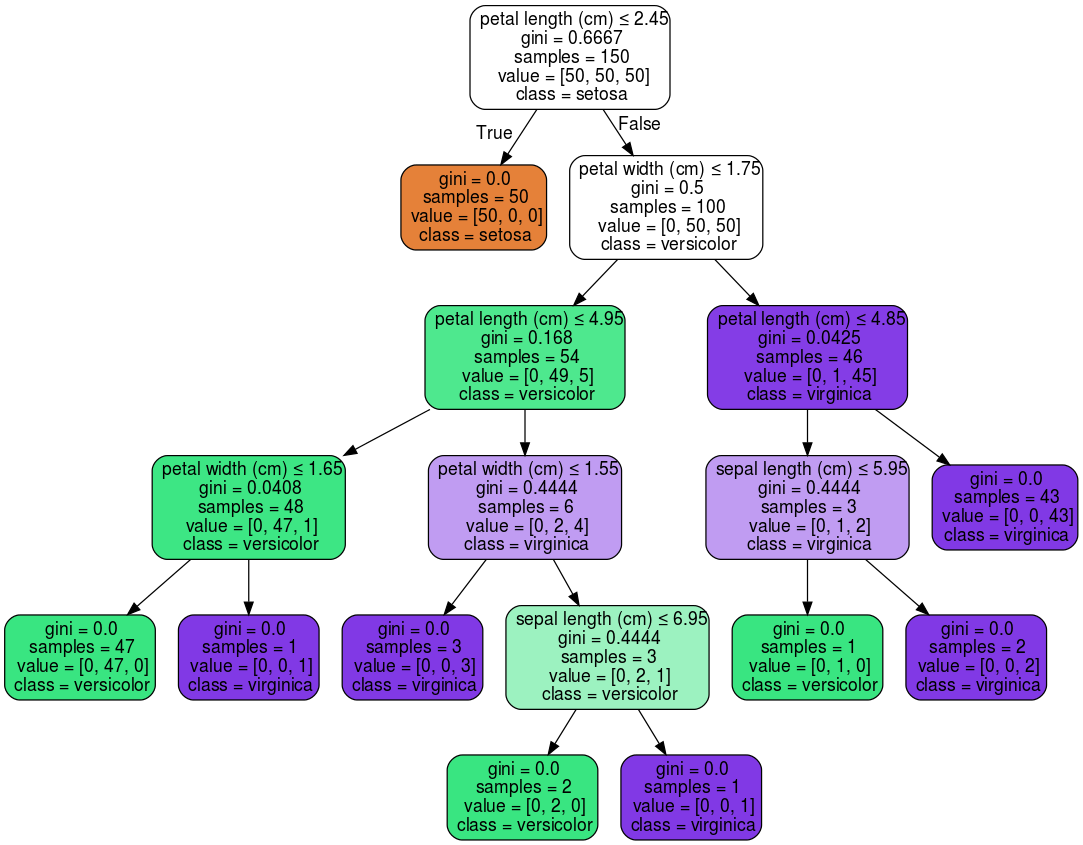
\includegraphics[scale=0.40]{figs/arvore-iris.png}
\label{f.arvore-iris}
\legend{\small Fonte: \cite{sklearn_api}.}
\end{figure}

Existem duas condições de parada para o algoritmos: as características possíveis para o problema se esgotarem, ou até que todas as instâncias das sub-regiões sejam pertencentes a uma mesma classe. \cite{James:2014:ISL:2517747}

Apesar deste método ser bem vantajoso por ser facilmente entendível e interpretável, infelizmente não são muito robustos por ser muito suscetível a perdas de precisão causadas por pequenas mudanças nas características, além de serem mais suscetíveis a \textit{overfitting}. 

\subsubsection{Florestas Aleatórias}

Florestas aleatórias é um método baseado em Árvores de Decisão. O algoritmo funciona com base em um número n, que determina quantas árvores são criadas, e para cada árvore n é selecionado de maneira aleatória um subconjunto de p características que esta árvore utilizará, considerando um número t de total de características. De maneira geral, o valor de p é calculado através de p = raiz quadrada de t. \cite{James:2014:ISL:2517747}

Este procedimento é muito eficiente, pois ao fazer com que as árvores sejam criadas com um número reduzido de características, elimina-se a possibilidade de que uma que seja muito mais forte do que as outras influencie tanto no resultado, de maneira que as árvores geradas sejam bem diferentes umas das outras e possuam um valor de variância mais alto entre elas. \cite{Breiman2001} 

Ao fim deste processo, as predições são feitas através de um sistema de votação. Os dados são passados por todas as árvores da floresta onde cada uma irá predizer uma classe, e enfim os votos serão contados e o resultado será definido pela classe com maior número de predições. 
Tomando como exemplo o caso de um sistema de classificação, que foi treinado por uma Floresta Aleatória de 100 árvores para separar suas entradas em duas classes X e Y. Cada entrada teria suas características processadas por todas as árvores e suas respectivas saídas obtidas. No caso de terem sido obtidos 60 predições de classe X e 40 predições de classe Y, essa entrada seria classificada como pertencente à classe X.

\begin{figure}[h]
\caption{\small Funcionamento de Florestas Aleatórias.}
\centering
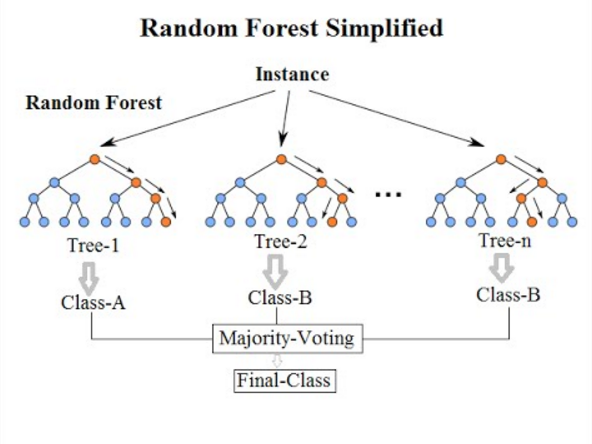
\includegraphics[scale=0.60]{figs/random-forests.png}
\label{f.random-forest}
\legend{\small Fonte: \cite{rfimagem}.}
\end{figure}

\subsubsection{AdaBoost}

AdaBoost, abreviação de \textit{Adaptive Boosting}, é um algoritmo formulado por \cite{FREUND1997119}, que busca melhorar a performance de outros classificadores. No contexto desse trabalho, será abordado a utilização deste algoritmo em conjunto com Árvores de Decisão.

O AdaBoost possui semelhanças com o algoritmo de Florestas Aleatórias, visto que ele busca trabalhar com um conjunto de classificadores de forma a obter um resultado mais confiável, porém se diferencia ao obter no final um modelo ao invés do modelo de votação anterior.

O algoritmo funciona mantendo um valor de peso $w_{i}$ para cada dado do conjunto de treino passado para o algoritmo. Depois, são feitas várias iterações aonde em cada uma é gerado um novo classificador fraco, que é o nome dado a um modelo que possui uma performance minimamente maior comparado a um algoritmo totalmente randômico, que possui acurácia próxima de 50 por cento.

É feita então uma predição com base neste algoritmo, e os pesos das variáveis são atualizados de acordo com o valor obtido pelo classificador, de maneira que se um dado foi classificado de maneira correta, seu peso diminui, e seu peso aumenta em caso contrário \cite{rojas2009adaboost}. Depois disso, o subconjunto utilizado pelo próximo classificador fraco é escolhido com base nos valores dos pesos.

\begin{figure}[h]
\caption{\small Funcionamento do AdaBoost.}
\centering
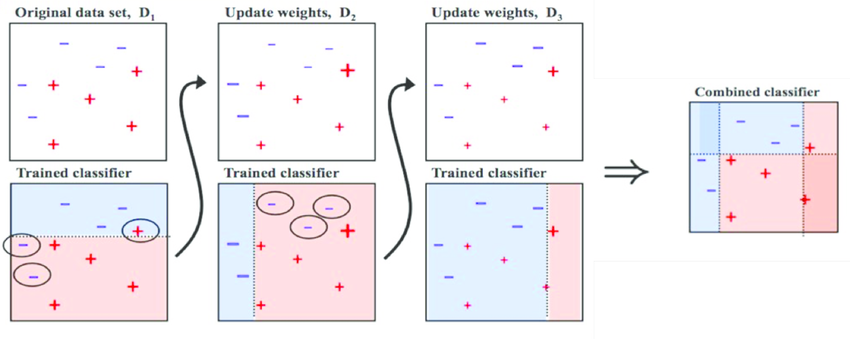
\includegraphics[scale=1.4]{figs/adaboost.png}
\label{f.adaboost}
\legend{\small Fonte: \cite{adaboost}.}
\end{figure}

Dessa maneira, o AdaBoost consegue favorecer em seus treinamentos o uso de variáveis que são mais difíceis de serem classificadas corretamente, o que faz dele muito eficiente em identificar \textit{outliers}. Ao final do processo, um modelo robusto é gerado com base nos passos anteriores dos classificadores fracos.

\subsubsection{Recursive Feature Elimination}

O RFE é um algoritmo recursivo que busca encontrar um subconjunto ótimo de características para um classificador específico, através do proceso de atribuição de um ranking de importância de cada uma delas.

O algoritmo começa sua execução com todas as características do conjunto passado, cria um modelo com base nelas, e calcula a importância de cada uma para a execução e performance do modelo. \cite{muller2017introduction} Depois disso, o algoritmo elimina a característica que teve o menor valor de importância e repete o processo recursivamente.

Ao final da execução, o algoritmo seleciona as $n$ características mais bem colocadas em seu ranking, obtendo assim o melhor conjunto possível, sendo $n$ um número pré-definido. 

\section{Revisão Bibliográfica}

Como base para este estudo, foram utilizados principalmente dois artigos. O primeiro, \textit{Machine learning for identifying botnet network traffic} \cite{12d2f5d1eba245f7bc2acc7487941bd7}, faz um estudo comparativo entre vários estudos da área, separando-os de acordo com tipo de ML e protocolo estudado, e depois apresentando características de cada um. Desse estudo, foram obtidos os seguintes artigos como base:

\begin{table}[h]
\centering
\begin{tabular}{|p{4cm}|p{5cm}|p{3cm}|}
\hline
\textbf{\small Autor(es)} & \textbf{\small Classificadores usados} & \textbf{\small{Características utilizadas}}\\\hline
{\small \cite{livadas2006usilng}} & {\small Árvores de Decisão,
Naive Bayes, 
Redes Bayesianas} & {\small 10}\\\hline
{\small \cite{strayer2008botnet}} & {\small Árvores de Decisão, Naive Bayes, Redes Bayesianas} & {\small 16}\\\hline
{\small \cite{masud2008flow}} & {\small Árvores de Decisão, Naive Bayes, Redes Bayesianas, SVM, Árvores de Decisão com Boosting} & {\small 20}\\\hline
\end{tabular}
\caption{Estudos da área utilizados como base para escolha dos classificadores.}
\label{t.articles}
\end{table}

De acordo com essa tabela, foram obtidos os estimadores e características base deste trabalho, com algumas ressalvas. Nota-se que Redes Bayesianas se fazem presente em todos eles, no entanto as bibliotecas deste trabalho não possuem implementação deste algoritmo. Portanto, Florestas Aleatórias foi incluído como substituto, por também ter sido utilizado em estudos relacionados \cite{rna2}. 

Além disso, como não foi especificado nos trabalho quais técnicas de \textit{Boosted Decision Trees} e Naive Bayes foram utilizadas, optou-se pelo uso do AdaBoost e pelo teste de Naive Bayes Multinomial e Bernoulli, respectivamente.

O segundo estudo é o \textit{Towards Effective Feature Selection in Machine Learning-Based Botnet Detection Approaches} \cite{beigi2014towards}, que apresenta um estudo detalhado sobre as características de rede predominantes na área. Com base neste e nos estudos utilizados anteriormente, foram definidas quais delas seriam utilizadas. 

Em conjunto com estes, também foram observados outros estudos com base que também apresentaram a utilização dos mesmos conjuntos de características, como \cite{featureselection} e \cite{iscx1}.

Entre elas, têm-se:

\begin{itemize}
    \item IP/Port de Origem e Destino: Estas características são utilizadas para a identificação dos fluxos de rede maliciosos;
    \item Protocolo: utilizado principalmente para a etapa de filtragem de pacotes, diminuindo dessa maneira o volume de pacotes a serem processados pelo algoritmo. Por exemplo, no contexto de uma \textit{Botnet} que utiliza o protocolo UDP para comunicação, é possível então filtrar os fluxos para que contenham somente os que utilizam o mesmo;
    \item Duração: característica muito utilizada para identificação de todos os tipos de protocolos de \textit{Botnet}, tendo em vista que elas de maneira geral costumam ter dois tipos bem distintos de conexão, sendo uma conexão inicial bem rápida seguidas de sessões muito longas;
    \item Características de tamanho de fluxo: Nesta categoria, estão presentes o Total de Bytes/Bits/Pacotes , Bytes por Pacote e Tamanho Médio de \textit{Payload}. Estas características ajudam a distinguir o fluxo de uma \textit{Botnet} de um tráfico normal baseado no fato de que o tráfego de \textit{Botnets} costuma ser muito mais uniforme do que os outros, que apresentam comportamentos mais variados dependentes da aplicação;
    \item Características de tempo de conexão: Nesta categoria, estão presentes Média de pacotes/bits por segundo, Média e Variância do tempo entre transmissão de pacotes (IAT). São utilizadas pelos mesmos motivos das características de tamanho de fluxo, para distinguir pelo comportamento da rede os tráfegos de \textit{Botnet};
    \item IOPR/Porcentagem de pacotes enviados: IOPR representa a relação entre o número de pacotes que chegam sobre o número de pacotes que são enviados em uma conexão. Assim como a porcentagem de pacotes enviados, estas características estão ligadas a estudos que indicam que a relação entre pacotes enviados e recebidos em redes normais segue uma distribuição uniforme. Porém, como estudos como \cite{almgren2010tracking} indicam que em redes infectadas por agentes maliciosos esta relação costuma ser desbalanceada, e portanto, pode ser utilizada para identificação de \textit{Botnets}.
\end{itemize}

